\subsection{Beam line at Paul Scherrer Institute (PSI)}
\begin{frame}
	\frametitle{Beam line at Paul Scherrer Institute (PSI)}
	\begin{itemize}
		\setlength{\itemsep}{\fill}
		\item High Intensity Proton Accelerator (HIPA) at PSI (Cyclotron)
		\item \SI{590}{\mega\electronvolt} proton beam with beam current up to \SI{2.4}{\milli\ampere}
		\begin{itemize}
			\vspace*{4pt}
			\item \SI{\sim1.4}{\mega\watt} \ra most powerful proton accelerator in the world
		\end{itemize}
		\item using beam line $\uppi$M1 with \SI{260}{\mega\electronvolt} positive pions ($\uppi^+$)
		\item tunable rate from \SI{2}{\kilo\hertz} to \SI{10}{\mega\hertz}
	\end{itemize}
	\begin{figure}
		\centering
		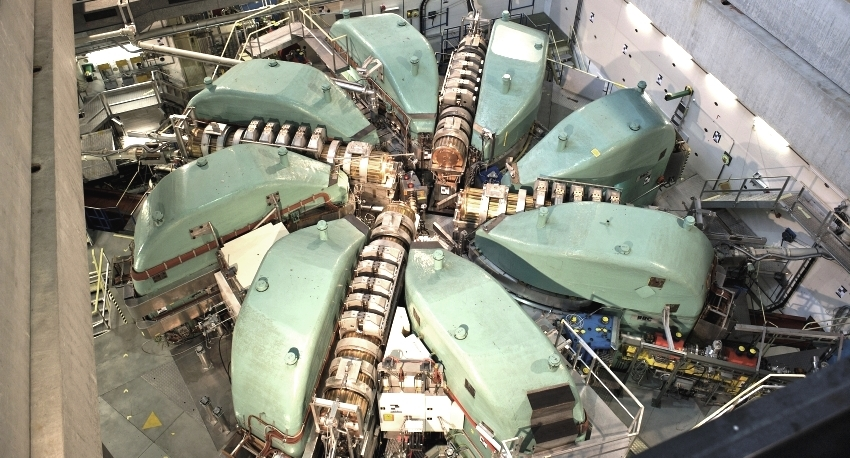
\includegraphics[width=7cm]{cyclotron}
	\end{figure}
\end{frame}
% ============================ new frame ==========================================>
\subsection{Overview}
\begin{frame}
	\frametitle{Overview}
	\begin{itemize}
		\item performing several beam tests starting in $2013$
		\item using a modular self-built beam telescope with two possible setups:
			\begin{itemize}
				\item pad setup (testing whole diamonds as single pad detector)
				\item pixel setup (testing diamond sensors implanted on CMS-Pixel Chips)
			\end{itemize}
		\item investigating several materials and devices
		\begin{itemize}
			\item scCVD pad detectors (reproduce rate effect)
			\item pCVD pad and pixel detectors
			\item very first 3D pixel detector
		\end{itemize}
		\item studying non-irradiated and irradiated devices (up to \SI{1e16}{neq\per cm^2})
	\end{itemize}
	\begin{figure}
		\centering
		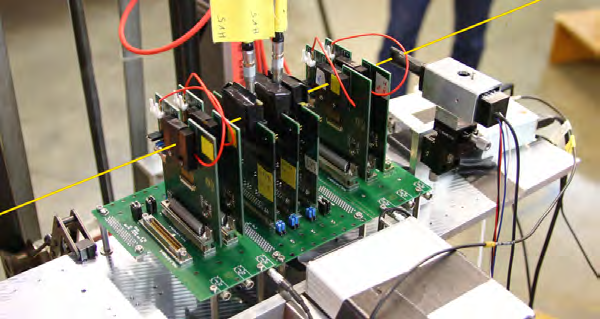
\includegraphics[width=6cm]{pad}
	\end{figure}
\end{frame}
% ============================ new frame ==========================================>
\subsection{Setup}
\begin{frame}
	\frametitle{Setup}
	\begin{figure}
		\centering
		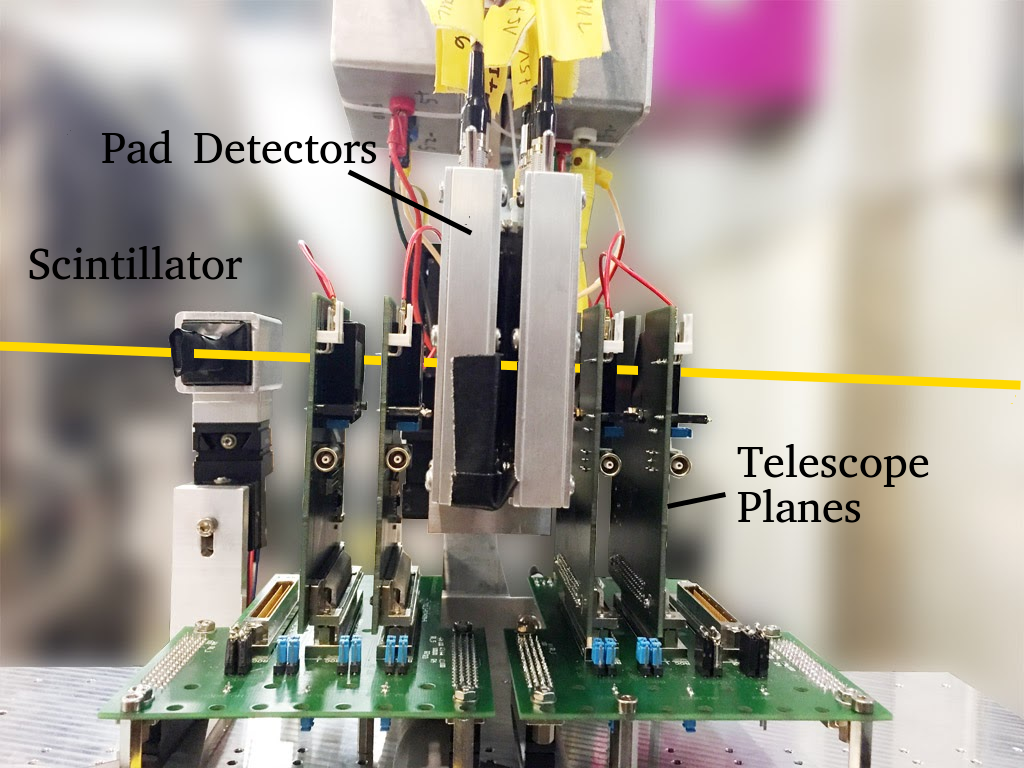
\includegraphics[width=5.5cm]{Setup}
	\end{figure}
	\begin{itemize}
		\setlength{\itemsep}{\fill}
		\item 4 tracking planes with analogue CMS pixel chips
		\item 2 diamond pad detectors
		\item scintillator for precise trigger timing: sigma of \SI{1.3\pm.1}{ns}
		\item resolution: \SI{\sim80x50}{\micro\meter}
	\end{itemize}
\end{frame}
% ============================ new frame ==========================================>
\begin{frame}
	\frametitle{Schematics}
	\begin{figure}
		\centering
		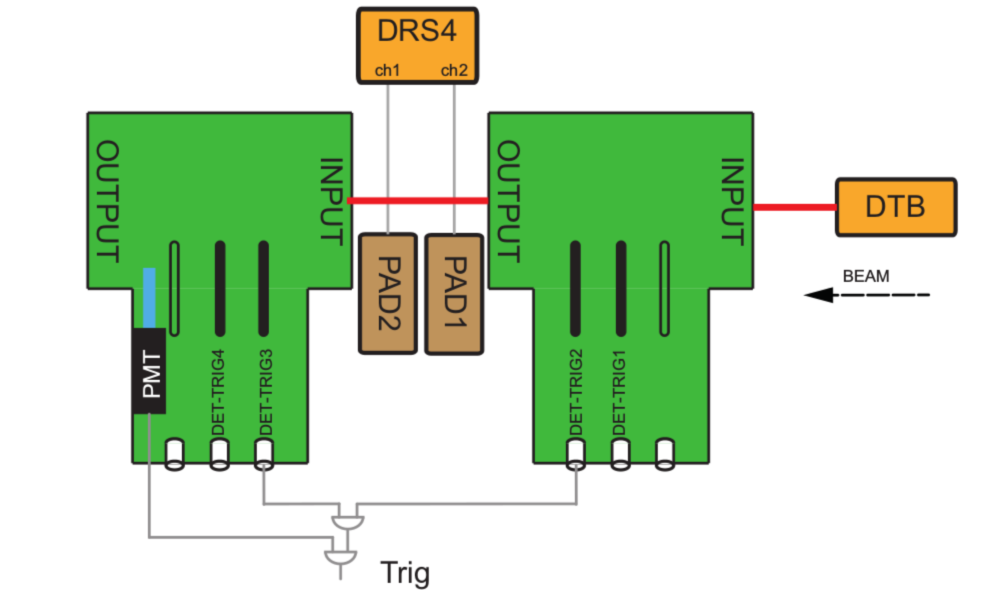
\includegraphics[width=7cm]{Schematics}
	\end{figure}
	\begin{itemize}
		\setlength{\itemsep}{\fill}
		\item using PSI DRS4 Evaluation Board as digitizer for the pad waveforms
		\item using Digital Test Board (DTB) and pXar software for the telescope readout
		\item global trigger as coincidence of fastOR self trigger and scintillator signal
		\item EUDAQ as DAQ framework
	\end{itemize}
\end{frame}
% ============================ new frame ==========================================>
\begin{frame}
	\frametitle{DAQ}
	\begin{figure}
		\centering
		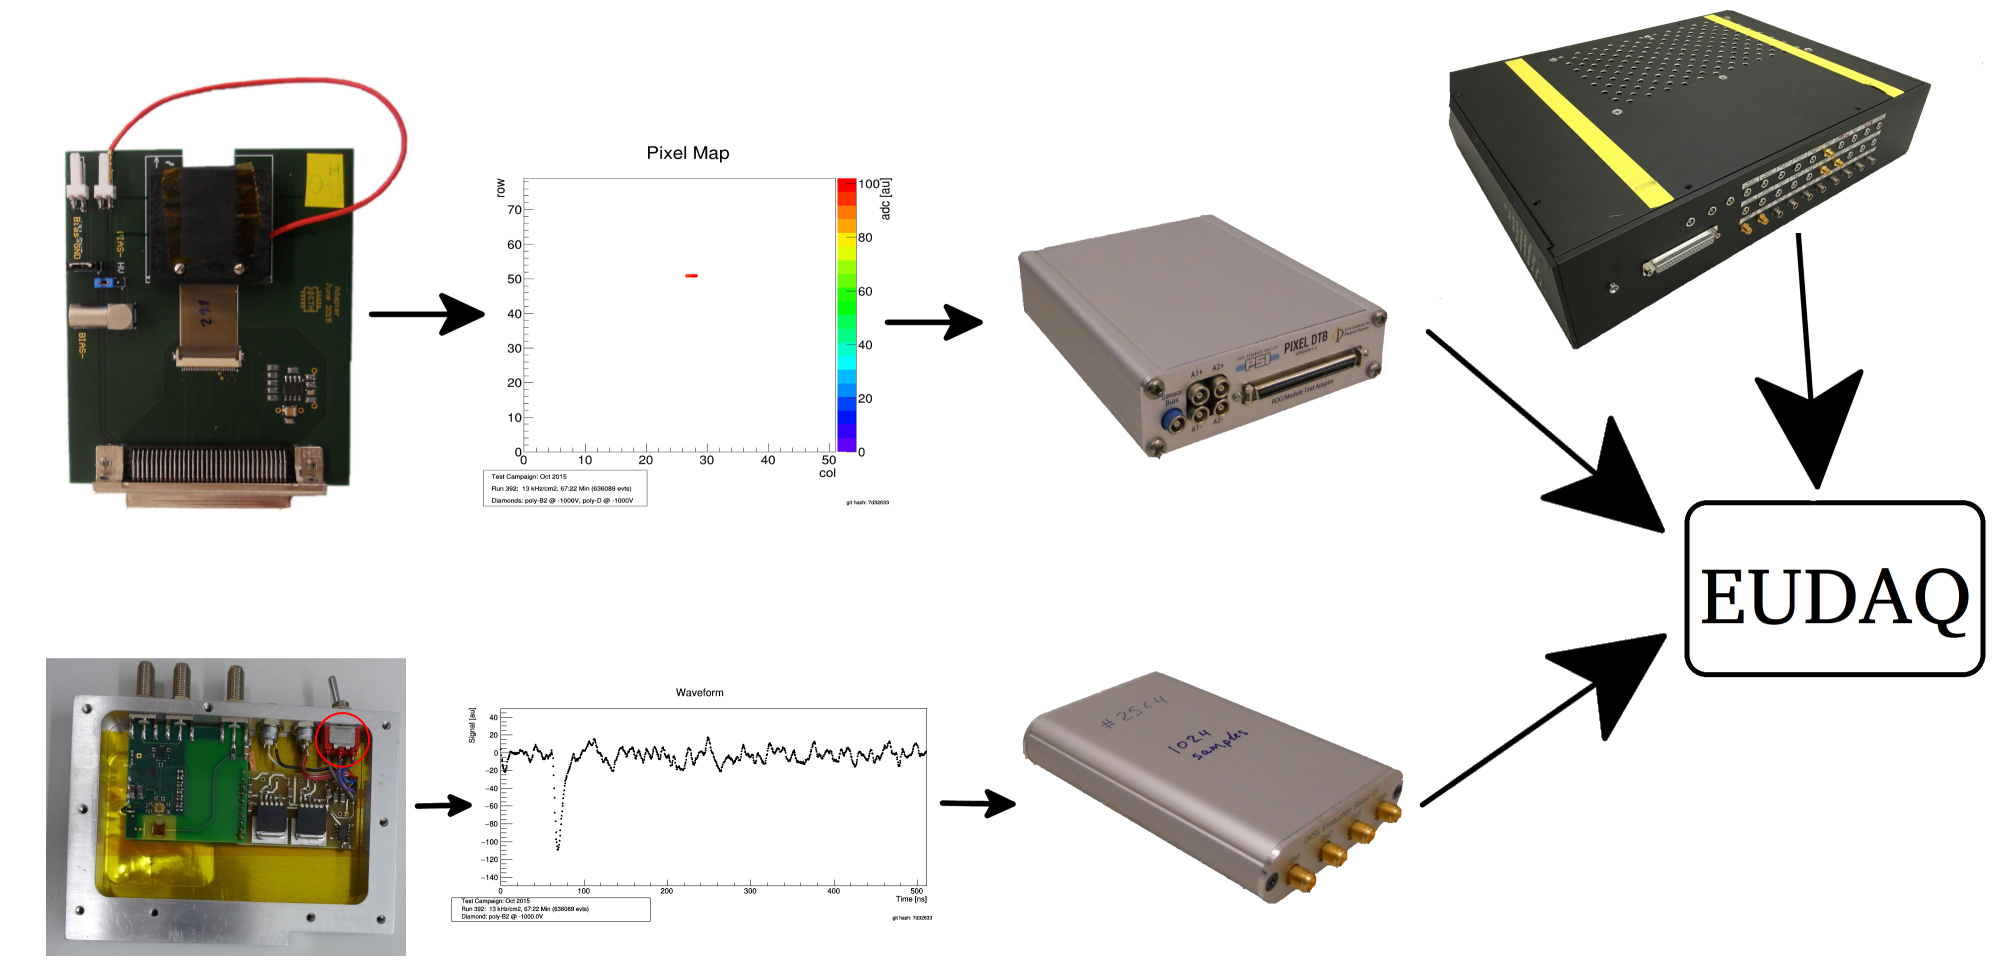
\includegraphics[width=.8\textwidth]{Intro}
	\end{figure}
	\begin{itemize}
		\item Trigger Unit to process the single triggers and provide global one for all devices
		\item EUDAQ saves event based data stream as binary file
	\end{itemize}
\end{frame}